% Chapter 1

\chapter{Introduction} % Write in your own chapter title
\label{Chapter:Intro}
\lhead{Chapter 1. \emph{Introduction}} % Write in your own chapter title to set the page header

\section{Motivation}
\label{sec:Motivation}

\subsection{The answer we seek.}
%Why did people first start looking at galaxies
The firmament has been the muse of humans for as long as we have recorded our history and most likely longer still. The field of astronomy is descended from the priests who worshiped celestial objects as the divine and sought them to bring meaning to their world. Structures such as Stonehenge use celestial objects to allow people to track the repetitious passage of time, thus being able to predict the seasons. Humanity became so convinced that universe was there for our benefit, elaborate orrerys with the earth at the center of all creation were built to explain how the sun and planets orbit around us. The progression to modern astronomy was slow and instead of assuming the universe was built for humans we now try to discover our place amongst a cosmos that is unfathomably enormous, diverse and inhospitable. 

The Milky Way is our home and was the first observed galaxy, the term comes from Greek to mean `milky circle' stemming from our belief that the universe exists to give us life and gives the galaxy a mammalian nurturing characteristic. The idea of complexity emerging from the universe is still present in the first classification of the structures of galaxies by Edwin Hubble \citep{Hubble1926Extra-galacticNebulae.,Hubble1927TheNebulae}. Complex spirals were thought to be the descendents of elliptical galaxies leading to the misnomer of 'early type' (elliptical) and 'late type' (spiral) galaxies, as it has since been found that it is in fact spiral galaxies that transform into elliptical galaxies.

Most of the aforementioned advances in astronomy have come from technological advances. When the most advanced way to view the cosmos was by simply looking upward we knew little of what there was and interpreted as best we could. With the advent of optics, such as lenses and then mirrors, leading to the building of telescopes the ability to look deeper into the heavens become a possibility and the first work on classification was done. Modern advances such as CCD/SED photographic plates, and telescopes that work outside of the visible light spectrum information, give information far beyond what the human eye can see. The more information we gather the more theories of formation come to be, the emergent complexity of Hubble gives way to hierarchical formation destroying structure, galaxies are found to be the birthplace of stars like our sun and where some galaxies are forming many stars some appear dead, looking backwards in time astronomers find the cosmos appears to have passed the peak of creation with galaxies on average forming less stars now then ever before. The one thing that connects all astronomers over all ages is the desire to answer the ultimate question of `why?'.

%How has the study of galaxies progressed
\subsection{The tools we use.}
The field of astronomy is somewhat unique in science in that all our data and `experiments' already exist it is simply up to us to seek them out. Often the hypothesis follows the data in contrary to the scientific method of collecting data to support a hypothesis. Furthermore, for galactic astronomers our objects are effectively frozen in time with the timescales galaxies evolve on eclipsing not only a human lifespan but the entirety of human civilization. It is our good fortune that the `cosmic speed limit', the speed of light, means the further away from earth we look the further back in time and into the history of galaxy formation. By looking at galaxies at many different epochs of cosmic time we are able to construct a picture of how the galactic population has changed. Theories of how the early universe transforms to the universe we see locally emerged and a tools were required to test these theories that could show galactic formation on human timescales. The first such model by \citet{Holmberg1941OnProcedure.} predates digital computing using an array of light bulbs using the `candle power' to proxy mass and evolving the system using gravitational arguments and confirms the hypothesis that in distributed merging systems the loss of energy during a encounter results in a capture or merger as we know it today.

With the rapid increase in computing power over the last century, the capability of the simulation of galaxies has grown. More than simply testing the dynamics of mass, simulations now have prescriptions for the formation of gas from stars, the mergers of complex systems of tens of galaxies in a full cosmological setting, the feedback of energy from central black holes millions of times tha mass of our sun, and more... \citep[e.g.,][]{McAlpine2015TheCatalogues, Pillepich2018FirstGalaxies}. However advance these models have become a full understanding of our Universe still seems to beyond our capability. Other less computationally intensive tools have been used to try to understand from first principles the formation of our Universe mathematical analytics have been proposed to model galaxies. Since their original inception where galaxies form via the loss of angular momentum and cooling of gas to form galactic disks \cite{Mo1998TheDiscs}, these so called Semi-Analytic Models have branched out to cover tens of different analytics that try to balance different processes to faithfully recreate as many observable galaxy properties as possible \citep[e.g.,][]{DeLucia2006TheGalaxies, Guo2011FromCosmology}. The most recent development in galactic modelling is more humble in it approach, seeing not to recreate the entire universe but use what we observe as a guide. These Semi-Empirical Models constrain the model as much as possible using observations and then ask focused questions to understand if our hypothesis of formation adequately link the observed galactic population over cosmic history \citep{Hopkins2010MERGERSMATTER, Zavala2012, Moster2013, Shankar2014, Moster2018Emerge10}.

%What questions will we answer
\subsection{The questions we answer.}
In this thesis I describe $\steel$, the STastical sEmi-Empirical modeL, as my contribution to the galactic modelling community. \steel has been designed to be in complement to the existing models of galaxy formation evolution and environment. \steel is biased on semi empirical modeling techniques but its defining characteristic is its statistical nature. Traditional models, described in more detail below, simulate: a cosmological volume, a catalogue of objects extracted from a cosmological volume, or a catalogue of objects generated to mimic a cosmological volume. \steel goes against this trend creating a simulation of the universe using number density functions to describe cosmological volumes without the volume and resolution constraint that effects discrete object simulations. The full methodology for \steel is given in Chapter \ref{Chapter:STEEL}. The advantage of having a volume free model is twofold, firstly, we can simulate rare objects that have a number density far lower than can be captured in traditional models, secondly, in a traditional model objects that appear with a high number density are simulated orders of magnitude more often than objects with low number density not only is this computationally inefficient it is a source of bias. 

\section{$\Lambda$CDM Cosmology}
\label{sec:LCDM}
%Why do we think dark matter exists
Dark Matter is a theorized form of matter that interacts only though gravity and is therefore not observable with traditional methods that rely on photons. The first notion of dark matter was from \citet{Zwicky1933DieNebeln}, it was observed that the binding mass required to hold the Coma Cluster together was roughly 400 times the observable stellar mass. It took many years and observations of the motions of satellites around our own galaxy also requiring an extended unseen matter structure until the ideas of dark matter begun to take hold. Further evidence was mounted by observing the rotation curves of galaxies \citep{Roberts1973ComparisonTypes}, the rotation of the outer regions of the galaxy did not fall off as the mass profile of the luminous galaxy should suggest. Whilst there exist other theories such as MOdified Newtonian Dynamics (MOND), that suggests gravity acts differently at large scales, dark matter is now the preferred model amoungst physicists to explain the mass deficit in the Universe. 

%What is LCDM
Once one accepts a type of matter that exits everywhere, is 5 times more abundant than baryonic matter, and does not appear to give out any electromagnetic signature the first logical question becomes ``What is it?''. To this day we do not know the precise nature of dark matter only some constraints to say what it is not. Initial thoughts suggested brown dwarf stars or black holes, dark yet familiar objects that satisfy both adding mass and not being visible. It is now thought that dark matter consists of a massive subatomic particle due to the proposed sizes of these particles they must inherently have a lower thermal velocity hence they became known as cold dark matter (CDM). By combining the formation model with the cosmological constant ($\Lambda$) to create a flat universe, \LCDM is born. 

%What are the predictions of LCDM
The prediction from \LCDM of foremost importance to galactic modelling is that of hierarchical assembly. Dark matter collapses under gravity from an initial density field, that mimics the cosmic microwave background. This means that areas of greater density collapse faster and eventually attract other collapsed regions further increasing their mass. This structure has become commonly referred to as the `cosmic web'. As dark matter interacts only via gravity it is relatively easy to simulate on large scales, as such there have been many massive simulations of \LCDM volumes in various cosmologies (WMAP5, Planck), of note are the Millennium simulation \citep{Boylan-Kolchin2009ResolvingSimulation} and the Bolshoi/MultiDark simulations \citep{Klypin2016}. I show a visulisation of the Bolshoi Plank dark matter simulation in \ref{fig:DMStruct}, the `cosmic web' is made visible dark matter halos seen here as the darkest regions are connected by filamentary structure. There is a notable void in the upper right of the image and two clusters one in the top middle and one in the bottom left. The initial dark matter distribution is accentuated by giga-years of collapse creating the complex structure seen.

\begin{figure}[h]
	\centering
	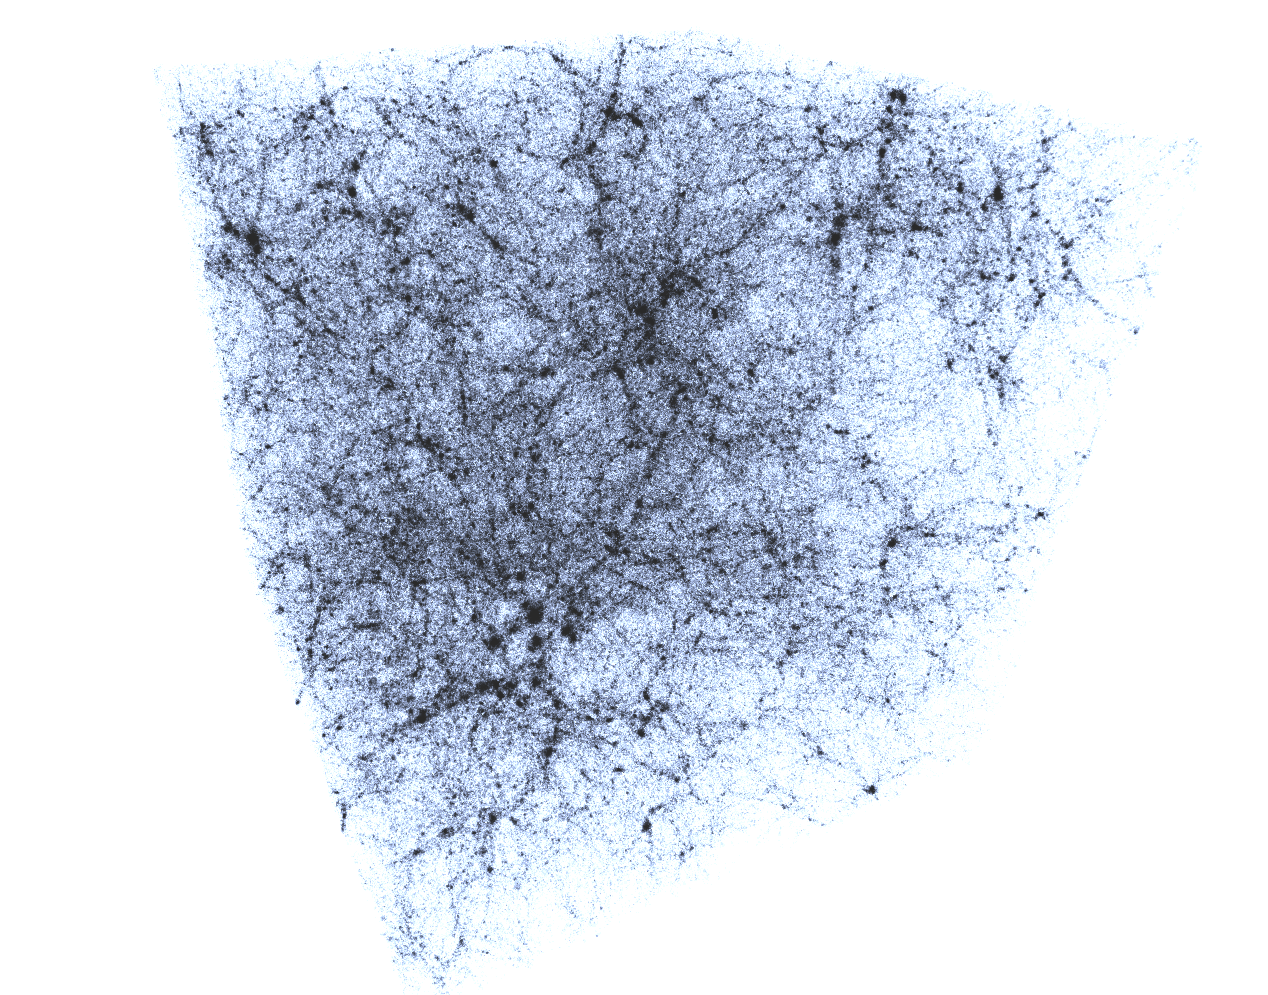
\includegraphics[width = \linewidth]{Figures/Chapter1/DMStruct.png}
    \caption{A visualization of the `cosmic web'. The shading shows the distribution of dark matter. The darkest regions are the spherical `halos' between the halos extended filaments can be seen. Regions of note are the void in the upper right and the clusters in the top middle and lower left, initially the dark matter density field would have been simmilar to the microwave background but giga-years of collapse have accentuated small features into large structure. Image Credit: C.Marsden using the galaxy and structure visualization code Astera processing the Bolshoi Planck dark matter simulation (https://astera.soton.ac.uk/).}
	\label{fig:DMStruct}
\end{figure}

%Halo Finders, Halo mass functions, Merger Trees and EPS formalism
To be able to analyze the complex dark matter structure objects must begin to be classified, the dark matter haloes, from simulations, that form the basis of many galaxy simulations are classified in two ways. Firstly, virialized haloes collections of dark matter particles\footnote{Note here a dark matter particle is a simulation element, often millions of solar masses, and not the theorized fundamental particle.} that are balanced in terms of their potential and kinetic energy, mathematically, 
\begin{equation}
    \langle T \rangle = -\frac{1}{2}\sum^{N}_{k=1}\langle \bold{F}_k \cdot \bold{r}_k \rangle.
\end{equation}
Secondly, haloes can be defined by their over density, simply with respect to either the background\footnote{The average density of the Universe.} or critical\footnote{The density required such that the universe will not expand forever.} density a spherical region is picked such that the average mass within this sphere is a set number times that density. For example $M_{200c}$ would be the mass of a halo where the halo is defined as the spherical region that is 200 times the critical density. It is then critical to gain an understanding of how these structures relate to one another. I have already introduced the concept of one halo growing though accretion of another, this is not an instantaneous process during accretion and subsequent cannibalization the smaller halo can be refereed to as a sub-halo. This creates collections of haloes in one space that are commonly referred to as groups or clusters depending on their mass or number of members. It is essential that these structures can be resolved from simulation and thus there have been several methods developed to analyze the simulated dark matter volumes to create catalogues of haloes. 

\begin{itemize}
    \item Bound Density Maximum: BDM classify halo structure by defining a spherical over density threshold e.g. $M_{200c}$ then removes particles that exceed the escape velocity \citep{Klypin1997Particle-MeshSimulations}.
    \item Friends of Friends: FOF uses a halo linking threshold, particles are `linked' together if they are closer than the threshold. One particle cannot be in two FOF groups simultaneously such that groups are unique, by assigning different linking lengths substructures can be identified and a picture of the halo hierarchy built \citep{Davis1985THEMATTER}.
    \item ROCKSTAR (Robust Overdensity Calculation using K-Space Topologically Adaptive Refinement): ROCKSTAR is a cutting edge development of the FOF halo finders, using a 6dimensional phase space and a temporal dimension the structure and evolution of haloes is extracted from dark matter simulations \citep{Behroozi2013TheCores}.
\end{itemize}

Once identified halos are then classified as central haloes or subhaloes, subhaloes then may contain further structure thus there are different `orders' of halos: $0^{th}$ order or central halos, $1^{st}$ order or sub-halos whose parent is a $0^{th}$ order halo, $2^{nd}$ order or sub-halos whose parent is a $1^{st}$ order halo, and so on. A useful description of the halo distributions are the halo and subhalo mass functions. The halo mass function is usually defined as the number density of central halos at a given mass in a given volume. The subhalo mass function has multiple definitions depending on the application, firstly, one can define the global subhalo mass function simmilar to the halo mass function this is the number density of subhaloes at a given mass in a given volume, secondly, one can define the subhalo mass function relative to a particular host halo to give the number of subhaloes of a given mass ratio $M_{subhalo}/M_{central}$ one expects to be associated to a halo mass $M_{central}$. As the subhaloes are an evolving population it is important to define which subhalo mass one is using:

\begin{itemize}
    \item Unevolved Subhalo Mass Function (USHMF): This mass function is the total number of subhaloes as a function mass that accreted onto a central halo over its entire history. The subhalo mass is added at the point of accretion and is never evolved and no number density is ever lost. This mass function is useful for understanding the total accretion history of a halo.
    \item Unevolved Surviving Subhalo Mass Function (USHMF): This mass function is the total number of subhaloes as a function mass that exist in a halo at a given epoch. Subhaloes once accreted are not updated in mass but do eventually merge and are then considered removed. This mass function is useful as it retains information about the infall mass and can be further broken down such that one knows the contribution of infall epochs.
    \item Evolved Subahlo Mass function (ESHMF): This mass function is the total number of subhaloes that exist in a halo at a given epoch where the subhaloes have undergone mass loss/transfer to the central halo. This mass function is the `true' subhalo mass function that one would expect to see if dark matter were directly observable.
\end{itemize}

In Figure \ref{fig:SubHaloes_byz} In the left hand panel I show the halo mass function at redshift $z=0.1$ note the characteristic shecter function shape with a linear relationship between number density and mass in log-log space that rapidly declines above a threshold mass, here $M_h\sim 10^{14}$ $M_{\odot}$. In the right hand panel I show the Global Unevolved Surviving Subhalo Mass Function at redshift $z=0.1$. In this figure the shading represents the redshift of infall, note the logarithmic scaling means the shading is not linear. Recent accretion is the dominant contributor of subhaloes at all masses, furthermore, for high mass subhaloes $M_h \geq 10^{13} M_{\odot}$ there is no contribution from high redshift accretion.

\begin{figure}[h]
	\centering
	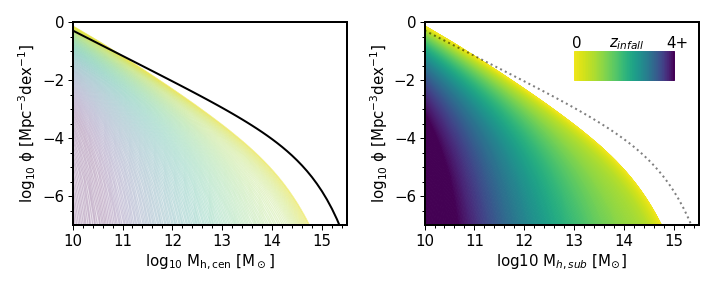
\includegraphics[width = \linewidth]{Figures/Chapter1/SubHaloes_byz.png}
    \caption{Left: I show the Halo Mass function, the global number density of haloes at redshift $z=0.1$. Right: I show the Global Unevolved Surviving Subhalo Mass Function at redshift $z=0.1$. The colour gradient shows the fraction of subhaloes at each mass contributed by redshift of infall, note due to the logarithmic scaling the thinner yellow bar at the top of the distribution is a majority contribution of subhaloes. There is a clear colour gradient from left to right showing that high mass haloes are exclusively contributed by recent accretion. In each panel I show the other mass function for comparison of number density.}
	\label{fig:SubHaloes_byz}
\end{figure}

In addition to the distinction between central and satellite haloes and their number densities information about the assembly is gained from simulations. Halo assembly histories are visualized as simple(ish) tree network, referred to as a merger tree. Central haloes are identified at a low redshift and the main progenitors followed backwards in time to create the central 'trunk', at any epoch where a merger occurs the main progenitor is assigned to be the larger of the two haloes\footnote{This remains true even if the main progenitor branch becomes smaller than the other branch at an earlier redshift.}. At each merger a 'branch' is created following this branch gives the history of that subhalo. In this way all the contributing haloes can be visualized. In Figure \ref{fig:SimpleTree} I give a example of a simple merger tree. There are increasingly more complex merger tree diagrams, it is not the case that a haloes merge simply I list some examples and show what these may look like on a stylized merger tree in Figure \ref{fig:Substructures}.

\begin{figure}[h]
	\centering
	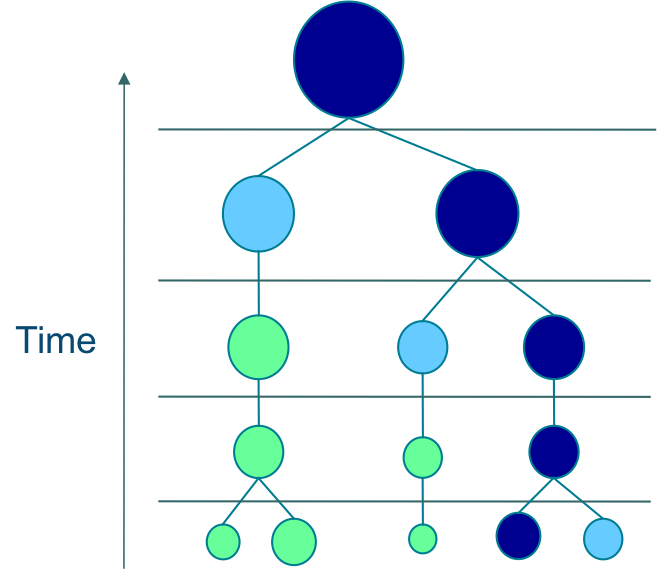
\includegraphics[width = \linewidth]{Figures/Chapter1/Merger_Tree_Simple.png}
    \caption{A cartoon of a simple merger tree. Forward time moves up the page as indicated on the right, horizontal lines separate epochs. Dark blue circles represent the main progenitor or trunk haloes of the merger tree. Haloes that merge directly onto the trunk are coloured in light blue, the merger history or branch for each of these merging haloes is shown in green.}
	\label{fig:SimpleTree}
\end{figure}

\begin{itemize}
    \item Substructure: A halo is not immediately dissolved upon accretion to the central halo, substructure is therefore maintained in central haloes between epochs. Furthermore, haloes on accretion may also carry substructure this creates 2nd (and above) order substructure.
    \item Flyby Haloes: Some haloes may pass through another halo and loose mass but not be fully captured. These haloes are known as flyby halos and must be accounted for to not over count accretion.
    \item Re-Accreted Haloes: Halos on particularly eccentric orbits or halos with initially high velocity may enter a halo and leave with a large velocity. These halos can then go to a distance where a simulation does not regard them as part of the halo group appearing to be flyby haloes. However, at some later time these halos may reenter the group. One must ensure these halos are not double counted, and that the mass they are accreted at is fir for purpose (i.e., mass at last accretion, mass at first accretion, or peak mass).
\end{itemize}

\begin{figure}[h]
	\centering
	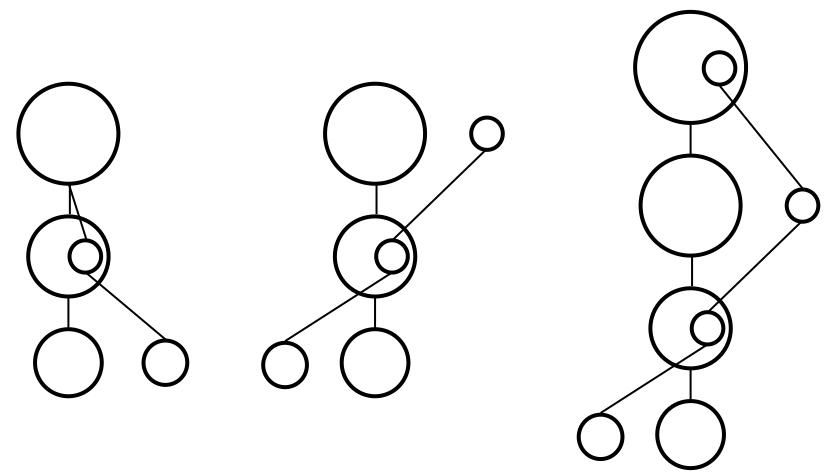
\includegraphics[width = \linewidth]{Figures/Chapter1/Substructures.png}
    \caption{From left to right: An example of, $1^{st}$ order substructure, a Flyby halo, a re-accreted halo.}
	\label{fig:Substructures}
\end{figure}

Whilst there is clearly a wealth of information in large dark matter simulations for many galaxy models that only require the simple dark matter distributions. Press-Schechter Formalism \citep{Press1974} provides an alternative way to generate simple analytic dark matter distributions. For a simple visualization one can consider the dark matter distribution at high redshift as a random Gaussian probability distribution, peaks in this distribution represent dark matter over densities and higher peaks collapse earlier. This can be visualized as a time evolving threshold above which the dark matter is a collapsed halo, if the summation of two gaussians are above this threshold then they are together are collapsed structure created by the merging of two haloes. A simple cartoon is shown to visualize this in Figure \ref{fig:PS_Cartoon}.

\begin{figure}[h]
	\centering
	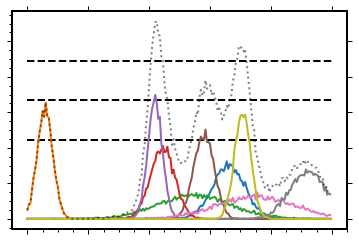
\includegraphics[width = \linewidth]{Figures/Chapter1/PS_Cartoon.png}
    \caption{A visualization of the core theory of Press-Schechter Formalism. The solid coloured lines are random gaussian distributions representing fluctuations in the initial mass density field, the grey dotted line is the total mass distribution, the three black dashed lines are for visualizing the threshold of collapse at different epochs.}
	\label{fig:PS_Cartoon}
\end{figure}

Following Figure \ref{fig:PS_Cartoon} considering the topped dashed line, as the first epoch we look for collapsed haloes, there are two peaks in the density field above the threshold the area above the threshold is related to the size of the halo and the spread the concentration. At the second threshold there is another collapsed peak mostly contributed by the brown gaussian that is close to a peak seen at the previous threshold from the yellow gaussian, furthermore, the two peaks from the first collapse have grown in mass as can be seen by an increased area. Finally, looking at the last collapse threshold,  on the left there is a new isolated peak more importantly on the right the peaks created by the yellow and brown gaussians now create one continuous area above the threshold this is an indication of two merged haloes, there are still two peaks that can be thought of in a simmilar manner to substructure. It is simple to see that at later epochs the merged substructures will also include the purple peak. This picture is a oversimplification of Press-Schechter Formalism, the gaussian field is actually significantly more interesting modeled from the CMB, instead of simple collapse thresholds a window function is used to smooth the density field. 

The Press-Schechter Formalism can be used to analytically build a merger tree by understanding the probability of any two over densities merging one can construct an algorithm that starting at a given redshift with a given mass halo and construct a theoretically valid merger history. I summarize here the \textsc{galform} \citep{Cole2000} method for making merger trees from Press-Schechter Formalism\footnote{In \citet{Parkinson2008GeneratingTrees} improvements to this method are proposed to better align the generated merger trees with the millennium simulation by using a perturbing function to remove systematic differences between N-Body simulations and the algorithm.}.

\begin{itemize}
    \item Pick a starting Mass, $M_{h}$ and redshift $z$. This will be the final mass/redshift for the main progenitor halo in the tree.
    \item Step backwards in redshift in steps, $dz$, where $dz$ is chosen that the probability, $P$, of a halo having a merger in $dz$ is $P\ll1$.
    \item Generate a uniform random number, $N$, if $N<P$ the halo splits, else the mass is reduced to account for unresolved haloes or smooth accretion and the process repeats.
    \item If the halo has split a random number is generated from the probability distribution that defines the possible progenitor halo masses from  Press-Schechter Formalism this is the mass of the split halo, $M_{split}$. The central halo mass is then updated to be less the split mass and a smooth/unresolved accretion component and the process repeated.
\end{itemize}

The merger trees generated using this algorithm are simpler and less computationally expensive and if calibrated properly fully consistent with \LCDM cosmology. They therefore are an ideal choice for simulations that need to generate halo merger trees on demand.

%How do these predictions effect galaxy assembly
Dark matter interacts with baryonic matter via gravity, as dark matter is 5 times more abundant than normal matter it is the dominant gravitational force in the universe, consequently a prediction of \LCDM cosmology is that the baryonic matter traces the dark matter distribution. Galaxies are thought to assemble in the center of dark matter halos where gas accumulates the larger the halo the larger quantity of gas collects in the halo and the larger the galaxy. The hierarchical assembly of dark matter halos is then translated into the galaxy population, massive galaxies are expected to be surrounded by many smaller satellite galaxies that loose angular momentum to the halo and eventually merge with the central galaxy.

\section{Hydrodynamic and N-Body Simulations}
\label{sec:Hydro}
%What is Hydrodynamics or N body
Hydrodynamical simulations are the most `real' galaxy simulation, dark matter, gas, and stars are assigned to a volume of particles and/or grid cells, forces are then applies to each element with respect to each other element. The volume is then solved by repeated solving and time stepping and snapshots produced at set intervals to be used for analysis. Processes that take place below the resolution limit of the simulation, such as starformation, are simulated using a sub-grid routine based on the properties of the given volume element.

%State of the Art
\subsection{State of the art: Illustris TNG}
The Illustris TNG simulations are a suite of 18 simulations, they use three different volumes, $\sim 50, 100, 300$ ${Mpc}^{3}$, and study a range of physical complexity and resolutions. TNG at its core use the code \textsc{arepo} \citep{Springel2010EMesh} which solves coupled ideal magneto-hydrodynamics and self gravity using periodic boundary conditions. Even for TNG50 where exceptionally high resolution for a cosmological simulation can be achieved much of the baryonic physics falls below the resolution limit, this physics in then included via so called `sub-grid' models. Sub-Grid models are used for star formation, super massive black holes, galaxy feedback process (starformation and AGN) and more. A specific example of one such sub-grid model is star formation, gas above a threshold density $n_H \simeq 0.1cm^{-3}$ is allowed to form stars following the results of \citet{Springel2003CosmologicalFormation}. Sub-grid models attempted to replicate results from smaller higher resolution simulations or from observations. 

\subsection{State of the art: FIRE}

%Drawbacks
\subsection{Pros and Cons}
The drawbacks of using a hydrodynamic model are foremost a limitation of resource they require vast amounts of computational resource to run and take a lot of developer time to create. Furthermore, they create huge amounts of output data that can be difficult to process and interpret. The combination of these effects result in a simulation that has volume and resolution constraints. For example the TNG simulations run three box sizes such that the larger boxes can simulate rare/low abundance objects and the smaller boxes can simulate galaxies in high detail, the computational time to run both would make the simulation impractical and the data products unmanageable. The advantages of this explicit modelling is that one can study the dynamics and interactions of the particles that make up galaxy directly, furthermore, by carefully choosing the size and resolution of the simulation it is possible to understand there details over many orders of magnitude. For example, in TNG one explores how the cosmological environment effects galaxy formation, the study of gas flow along dark matter filaments and understand the statistics of galaxy mergers. Alternately in FIRE one high resolution `zoom in' region is simulated with high fidelity, the resolution is such that feedback from starformation winds, AGN, and even individual supernovae are resolved. Whilst hydrodynamics represent the stare of the art in our ability to simulate a universe or a individual galaxy in a holistic manner the time and difficulty mean they are not the ideal tool for testing they cannot be easily re-run and are therefore not ideal as laboratories to test ideas. With the rapid progress in computational resource in terms of memory and speed and novel techniques such as genetic modification, the art of subtly altering the initial conditions to test how perturbations and modelling assumptions effect self simmilar galaxies \citep{Pontzen2017HowGalaxy}, it may well become possible to use hydrodynamic simulations as comprehensive tools, but as it stands we need faster and more flexible tools.  

\section{Semi-Analytic Modeling}
\label{sec:SAM}
%What is a SAM

%State of the art SAM

%Drawbacks of SAM

\section{Semi-Empirical Modelling}
\label{sec:SEM}
%What is a SEM

%State of the art SEM

%Drawbacks of SEM

\section{Galaxy Surveys Present and Future}
\label{sec:Surveys}
%First galaxy surveys

%SDSS

%COSMOS and CANDLES 

%Euclid


